\documentclass{standalone}
\usepackage{tikz}
% \usepackage{pgfmath}

\usepackage{calc}
\usetikzlibrary{intersections, calc}
\usepackage{hsbcommon}
% \def\myopacity{1}
    \begin{document}

% \def\myopacity{1}
    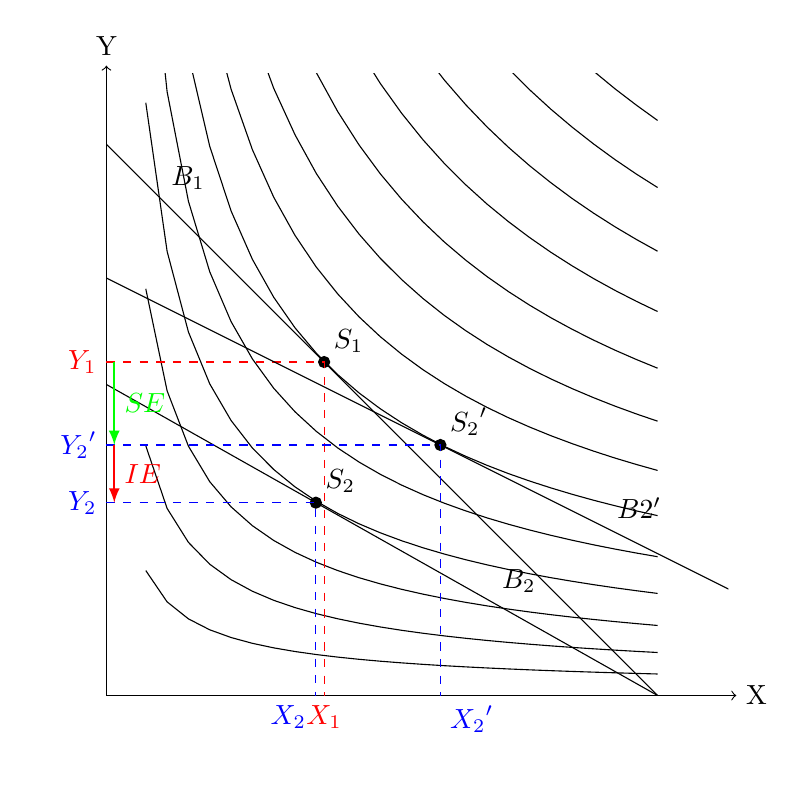
\begin{tikzpicture}[domain=0:8]
        
        \draw[->] (0,0) node[below] {\phantom{$X_i$}} -- (8,0) node[right]  {X};
        \draw[->] (0,0) node[left] {\phantom{$Y_mi$}} -- (0,8) node[above]  {Y};

        \def\myalpha{0.4}
        \def\mybeta{0.6}
        \def\myprice{0.5}
        \def\mycolor{black}

        \clip (-1,-1) rectangle (7.9,7.9);
        \foreach [count=\i] \niveau in {1,1.515,...,8}
            {
            % \pgfmathparse{int(mod(\i,5))}% mod 5 => every fifth
            % \edef\mycolor{\ifnum\pgfmathresult=3 red\else white\fi}
            \draw[domain=0.5:7, name path=indiff\i,color=\mycolor] plot (\x, {(\niveau/\x^\myalpha)^(1/\mybeta)}); 
}
        \coordinate (A) at (0,7);
        \coordinate (C) at (7,0);

        \draw[name path=budget1] (A) -- (C);
            \node[above right] at ($(A)!0.1!(C)$) {$B_1$}; 
            \coordinate (S1) at ($(A)!0.395!(C)$); %% optischer tangentialpunkt
            \filldraw (S1) node[above right] {$S_1$} circle (2pt) ;
            % \draw (0, |- A) -- (A) -- (|- A, 0);
            \draw[dashed,red]  (0, |- S1) node[left] {$Y_1$} -- (S1) -- (S1 |-,0) node[below] {$X_1$};            

        %% One price doubles
        \coordinate (B) at (0,3.95);
        \ifstep{1}{

            \draw[name path=budget2] (B) -- (C);
                \node[above right] at ($(B)!0.7!(C)$) {$B_2$}; 
                \coordinate (S2) at ($(B)!0.38!(C)$); %% optischer tangentialpunkt
                \filldraw (S2) node[above right] {$S_2$} circle (2pt) ;
                \draw[dashed,blue]  (0, |- S2) node[left] {$Y_2$}-- (S2) -- (S2 |-,0) node[below left] {$X_2$};                 
        }

        %% moving the new budget line
        \def\incomeeffect{1.515}
        \coordinate (D) at (0,7*\myprice*\incomeeffect);
        \coordinate (E) at (7*\incomeeffect,0);
        \ifstep{2}{

            \draw (D) -- (E);
                \node[above right] at ($(D)!0.6!(E)$) {$B2'$}; 
    
            \coordinate (S3) at ($(D)!0.4!(E)$); %% optischer tangentialpunkt
                \filldraw (S3) node[above right] {${S_2}'$} circle (2pt) ;
                \draw[dashed,blue]  (0, |- S3) node[left] {${Y_2}'$}-- (S3) -- (S3 |-,0) node[below right] {${X_2}'$};      
        }

        %% showing the size of the effect
        \ifstep{3}{

            \draw[->,>=latex,thick,green] (0.1,|- S1) -- node [right] {$SE$} (0.1, |- S3) ;
            \draw[->,>=latex,thick,red] (0.1,|- S3) -- node [right] {$IE$} (0.1, |- S2) ;

            % \draw[->,>=latex,thick,green] (S1 |-,0.1 ) -- node [below] {$SE$} (S3 |- , 0.1) ;
            % \draw[->,>=latex,thick,red] (S3 |-,0.2) -- node [above] {$IE$} (S2 |-, 0.2) ;
        }

        
        % %% moving old budget line
        % \def\slutsky{0.5}
        % \def\slutskyeffect{1.32}
        % \coordinate (F) at (0,7*\slutsky*\slutskyeffect);
        % \coordinate (G) at (7*\slutsky*\slutskyeffect,0);
        % \ifstep{4}{

        %     \draw (F) -- (G);
        %         \node[above right] at ($(F)!0.6!(G)$) {$B2'$}; 
    
        %     \coordinate (S4) at ($(F)!0.4!(G)$); %% optischer tangentialpunkt
        %         \filldraw (S4) node[above right] {${S_4}'$} circle (2pt) ;
        %         \draw[dashed,blue]  (0, |- S4) node[left] {${Y_2}''$}-- (S4) -- (S4 |-,0) node[below right] {${X_2}''$};      
        % }

    \end{tikzpicture}
\end{document}
